\documentclass[aspectratio=169,12pt]{beamer}

% Theme and colors
\usetheme{Madrid}
\usecolortheme{dolphin}
\usefonttheme{professionalfonts}

% Packages
\usepackage{amsmath,amssymb}
\usepackage{graphicx}
\usepackage{booktabs}
\usepackage{tikz}
\usepackage{xcolor}
\usepackage{multirow}
\usepackage{adjustbox}
\usepackage{pgfpages}

% =====================================
% PRESENTATION MODE OPTIONS
% =====================================
% Uncomment ONE of the following options:

% Option 1: Standard presentation (no notes)
% No additional settings needed

% Option 2: Presentation with notes on second screen (for presenter)
%\setbeameroption{show notes on second screen=right}

% Option 3: Print version with notes
%\setbeameroption{show notes}

% Option 4: Handout version (4 slides per page, no notes)
%\usepackage{pgfpages}
%\pgfpagesuselayout{4 on 1}[a4paper,border shrink=5mm,landscape]

% Option 5: Handout with notes (2 slides + notes per page)
%\usepackage{pgfpages}
%\pgfpagesuselayout{2 on 1}[a4paper,border shrink=5mm]
%\setbeameroption{show notes}
% ====================================

% Remove navigation symbols
\setbeamertemplate{navigation symbols}{}

% Set bullet points
\setbeamertemplate{itemize items}[circle]
\setbeamertemplate{enumerate items}[default]

% Title information
\title[JointODE]{Joint Modeling of Longitudinal and Survival Data via Second-Order ODEs}
\subtitle{A Mechanistic Approach to Biomarker Dynamics and Event Risk}
\author{Ziyang Gong}
\institute{}
\date{September 2025}

% Define colors
\definecolor{myblue}{RGB}{0,62,126}
\definecolor{mygreen}{RGB}{0,128,0}

\begin{document}

% Title slide
\begin{frame}
  \titlepage
  \note{

    \small
    [Time: 1 min | Total: 1 min]

    Good afternoon, everyone. Thank you for joining me today.

    I'd like to present our work on a new approach to joint modeling. We use
    second-order differential equations to model longitudinal biomarker data
    together with survival outcomes.

    Our central question is this: Can we improve risk prediction by modeling
    not just biomarker levels, but also their velocities - how fast they're
    changing?

    I'll walk you through our methodology, show some preliminary results, and
    would very much appreciate your feedback.
    \normalsize
  }
\end{frame}

% Section 1: Motivation
\section{Motivation}

\begin{frame}{Motivating Example: PSA Velocity in Prostate Cancer\footnotemark[1]}
  \textbf{Goal:} Joint modeling of biomarker trajectories and survival outcomes.

  \vspace{0.3cm}
  \begin{columns}[T]
    \begin{column}{0.45\textwidth}
      \textbf{PSA Kinetics - Patient A}
      \begin{itemize}
        \item Baseline PSA: $4.0$ ng/mL
        \item PSA velocity: $0.35$ ng/mL/year
        \item Pattern: Stable rise
        \item \textcolor{green}{Low risk progression}
      \end{itemize}
    \end{column}

    \begin{column}{0.45\textwidth}
      \textbf{PSA Kinetics - Patient B}
      \begin{itemize}
        \item Baseline PSA: $4.0$ ng/mL
        \item PSA velocity: $2.0$ ng/mL/year
        \item Pattern: Rapid rise
        \item \textcolor{red}{High risk progression}
      \end{itemize}
    \end{column}
  \end{columns}

  \vspace{0.5cm}
  \begin{center}
    \Large
    Can we leverage biomarker velocity to improve risk prediction?
  \end{center}

  \footnotetext[1]{\scriptsize D'Amico AV, et al. JAMA. 2005;294(4):440-447.}
  \note{

    \footnotesize
    [Time: 2.5 min | Total: 3.5 min]

    Let me start with a motivating example from clinical practice.

    Consider two prostate cancer patients. Both have PSA levels of four point zero
    nanograms per milliliter today. Looking at just this snapshot, they seem
    identical.

    But here's the key difference: Patient A's PSA rises at zero point three five units per
    year, while Patient B's increases at two point zero per year - nearly six times
    faster.

    Clinically, these patients require very different management. Patient B
    needs more aggressive intervention.

    This raises an important statistical question: How can we formally
    incorporate this velocity information into our models? Traditional joint
    models focus primarily on current levels. We hypothesized that explicitly
    modeling velocity could enhance predictive accuracy.
    \normalsize
  }
\end{frame}

\begin{frame}{Our Solution: Mechanistic Modeling via ODEs}
  \textbf{Second-order ODE framework for biomarker dynamics:}
  \begin{equation*}
    \boxed{\ddot{m}(t) + 2\xi\omega\dot{m}(t) + \omega^2 m(t) = k\omega^2 u(t)}
  \end{equation*}
  $\xi$: damping ratio, $\omega$: natural frequency, $k$: gain, $u(t)$: excitation

  \only<1>{
    \begin{figure}
      \centering
      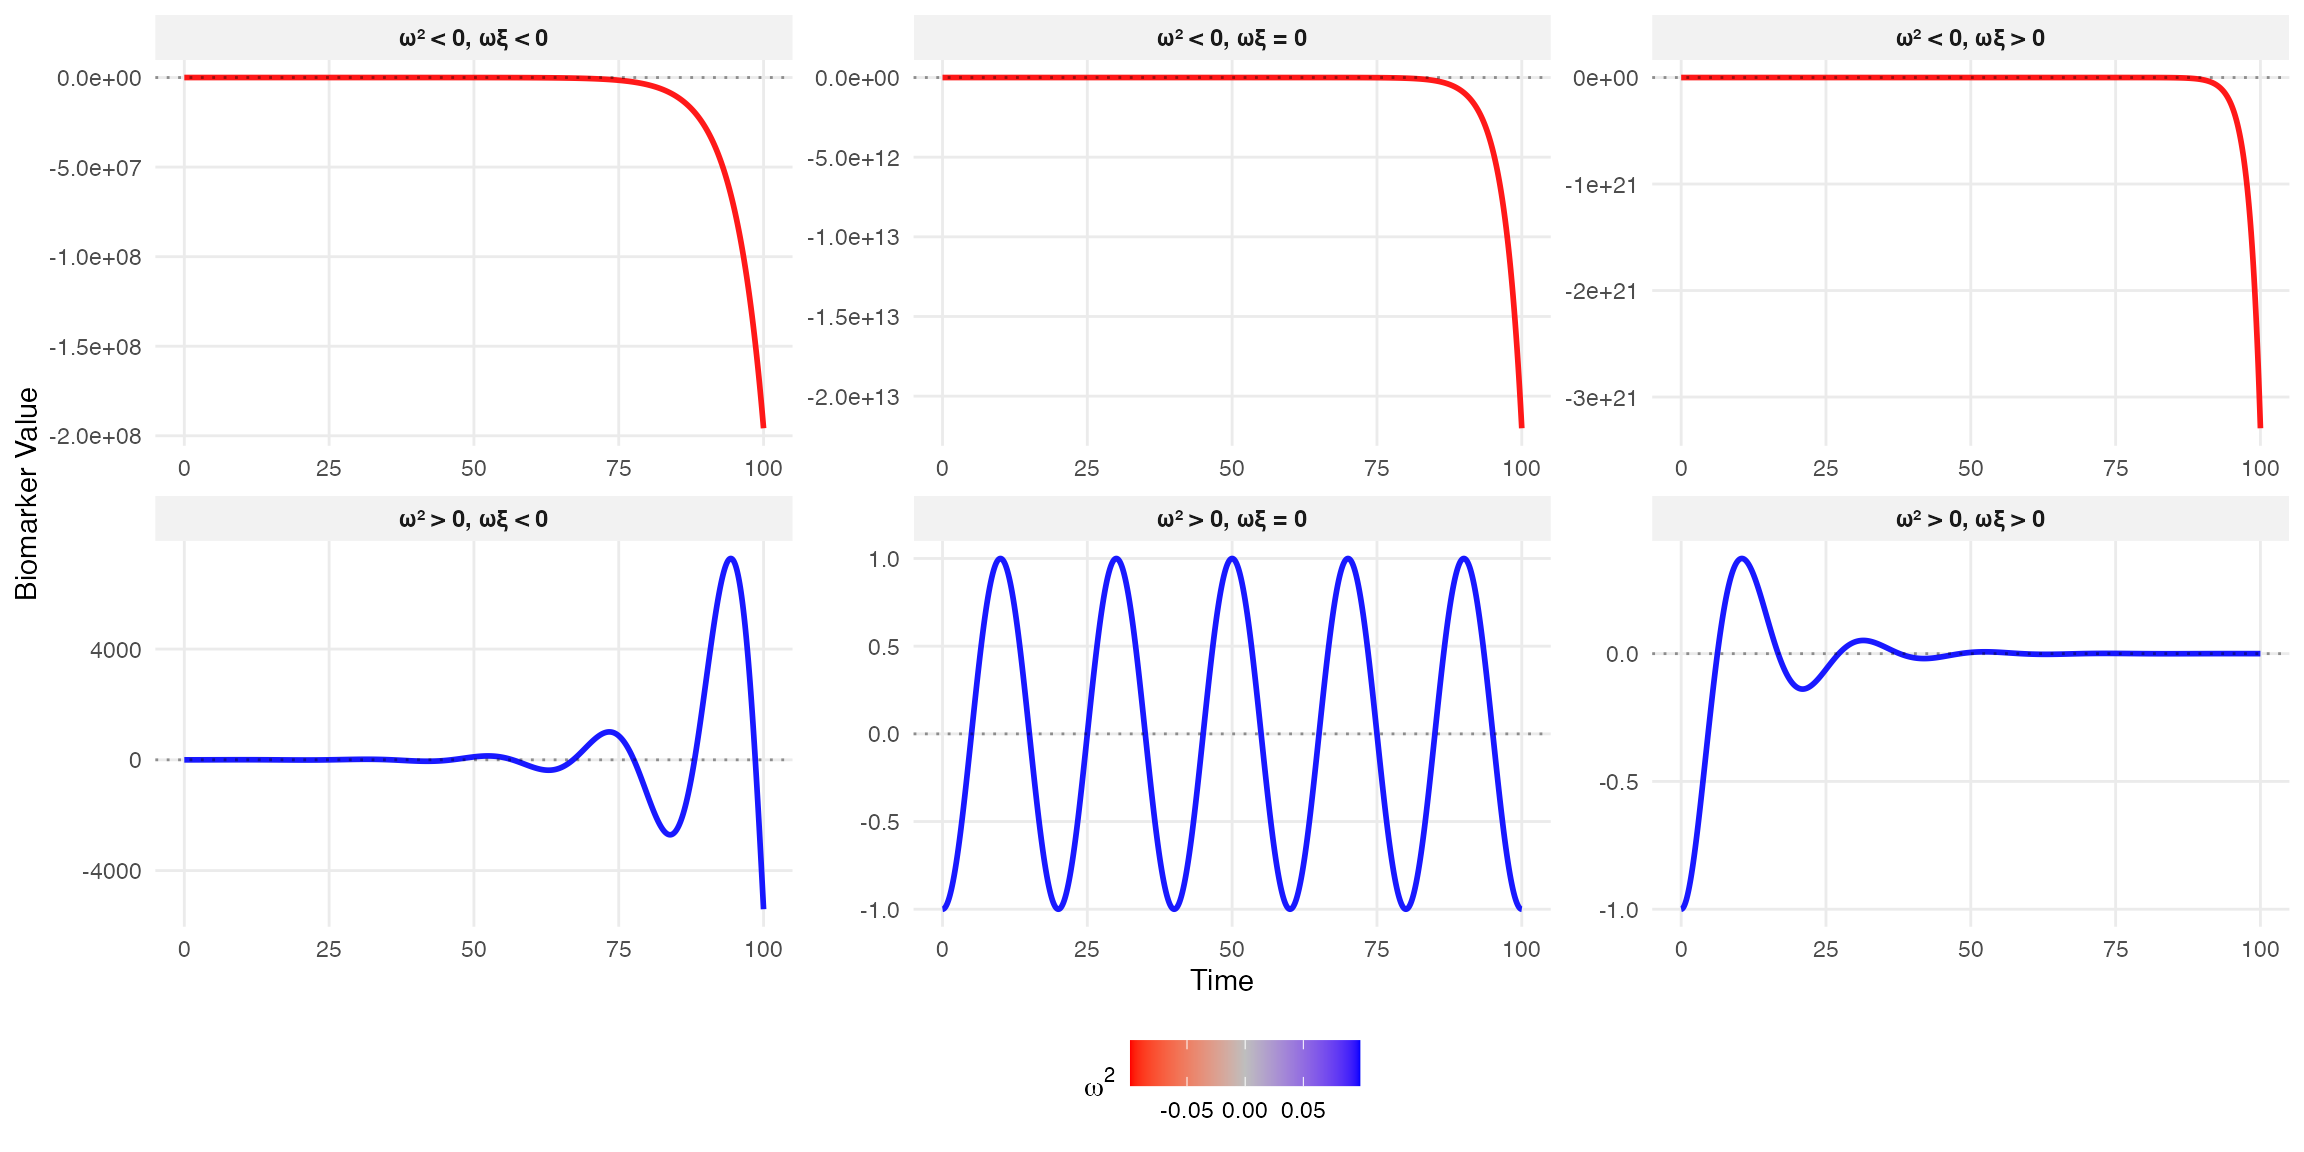
\includegraphics[width=0.7\textwidth]{../../docs/articles/illustration_files/figure-html/dynamic-cases-1.png}
    \end{figure}
  }
  \only<2>{
    \vspace{0.3cm}
    \textbf{Stability Conditions:}
    \begin{itemize}
      \item \textbf{Stable:} $\omega^2 > 0$ and $\omega\xi > 0$
      \item \textbf{Unstable:} $\omega^2 \leq 0$ or $\omega\xi \leq 0$
    \end{itemize}

    \vspace{0.3cm}
    Can we test $H_0: \omega^2 \leq 0$ or $\omega\xi \leq 0$ vs $H_1: \omega^2 > 0$ and $\omega\xi > 0$?

  }
  \note{

    \tiny
    [Time: 3.5 min | Total: 7 min]

    We adopt second-order ODEs from engineering - and it turns out they're
    remarkably natural for modeling biological systems.

    Look at the diversity of trajectories (tra-JECK-tor-eez) in this figure.
    These aren't just abstract mathematical curves - we observe exactly these
    patterns in real data: oscillatory behavior, smooth convergence to
    equilibrium, and divergent trajectories (tra-JECK-tor-eez).

    Just three
    parameters capture the entire dynamics:
    - omega: The natural frequency - how quickly the system responds
    - xi (ksai): The damping ratio - whether we get oscillations
      or smooth decay
    - k u(t): The equilibrium level - where the biomarker is heading

    Now here's what makes ODEs particularly powerful: velocity comes for free.
    Traditional methods require numerical differentiation. But when we solve the ODE, we automatically get both the biomarker
    level and its rate of change.

    But there's more. We discovered that stability itself carries medical meaning.
    Stable trajectories (tra-JECK-tor-eez) indicate treatment is working, like this blue one here, while
    unstable ones signal trouble - perhaps resistance or progression, like the other curves.

    [Click 2]
    The mathematics provides precise stability conditions: we need omega-squared
    greater than zero and omega-times-xi greater than zero.

    But here's where it gets exciting: when these stability conditions fail,
    trajectories (tra-JECK-tor-eez) diverge. We can test for this instability in the data. However this is not today's focus. Maybe in future work. Today, I'll focus on the use of velocity in risk prediction.
  
    \normalsize
  }
\end{frame}


\begin{frame}{Damping Effects}
  \begin{figure}
    \centering
    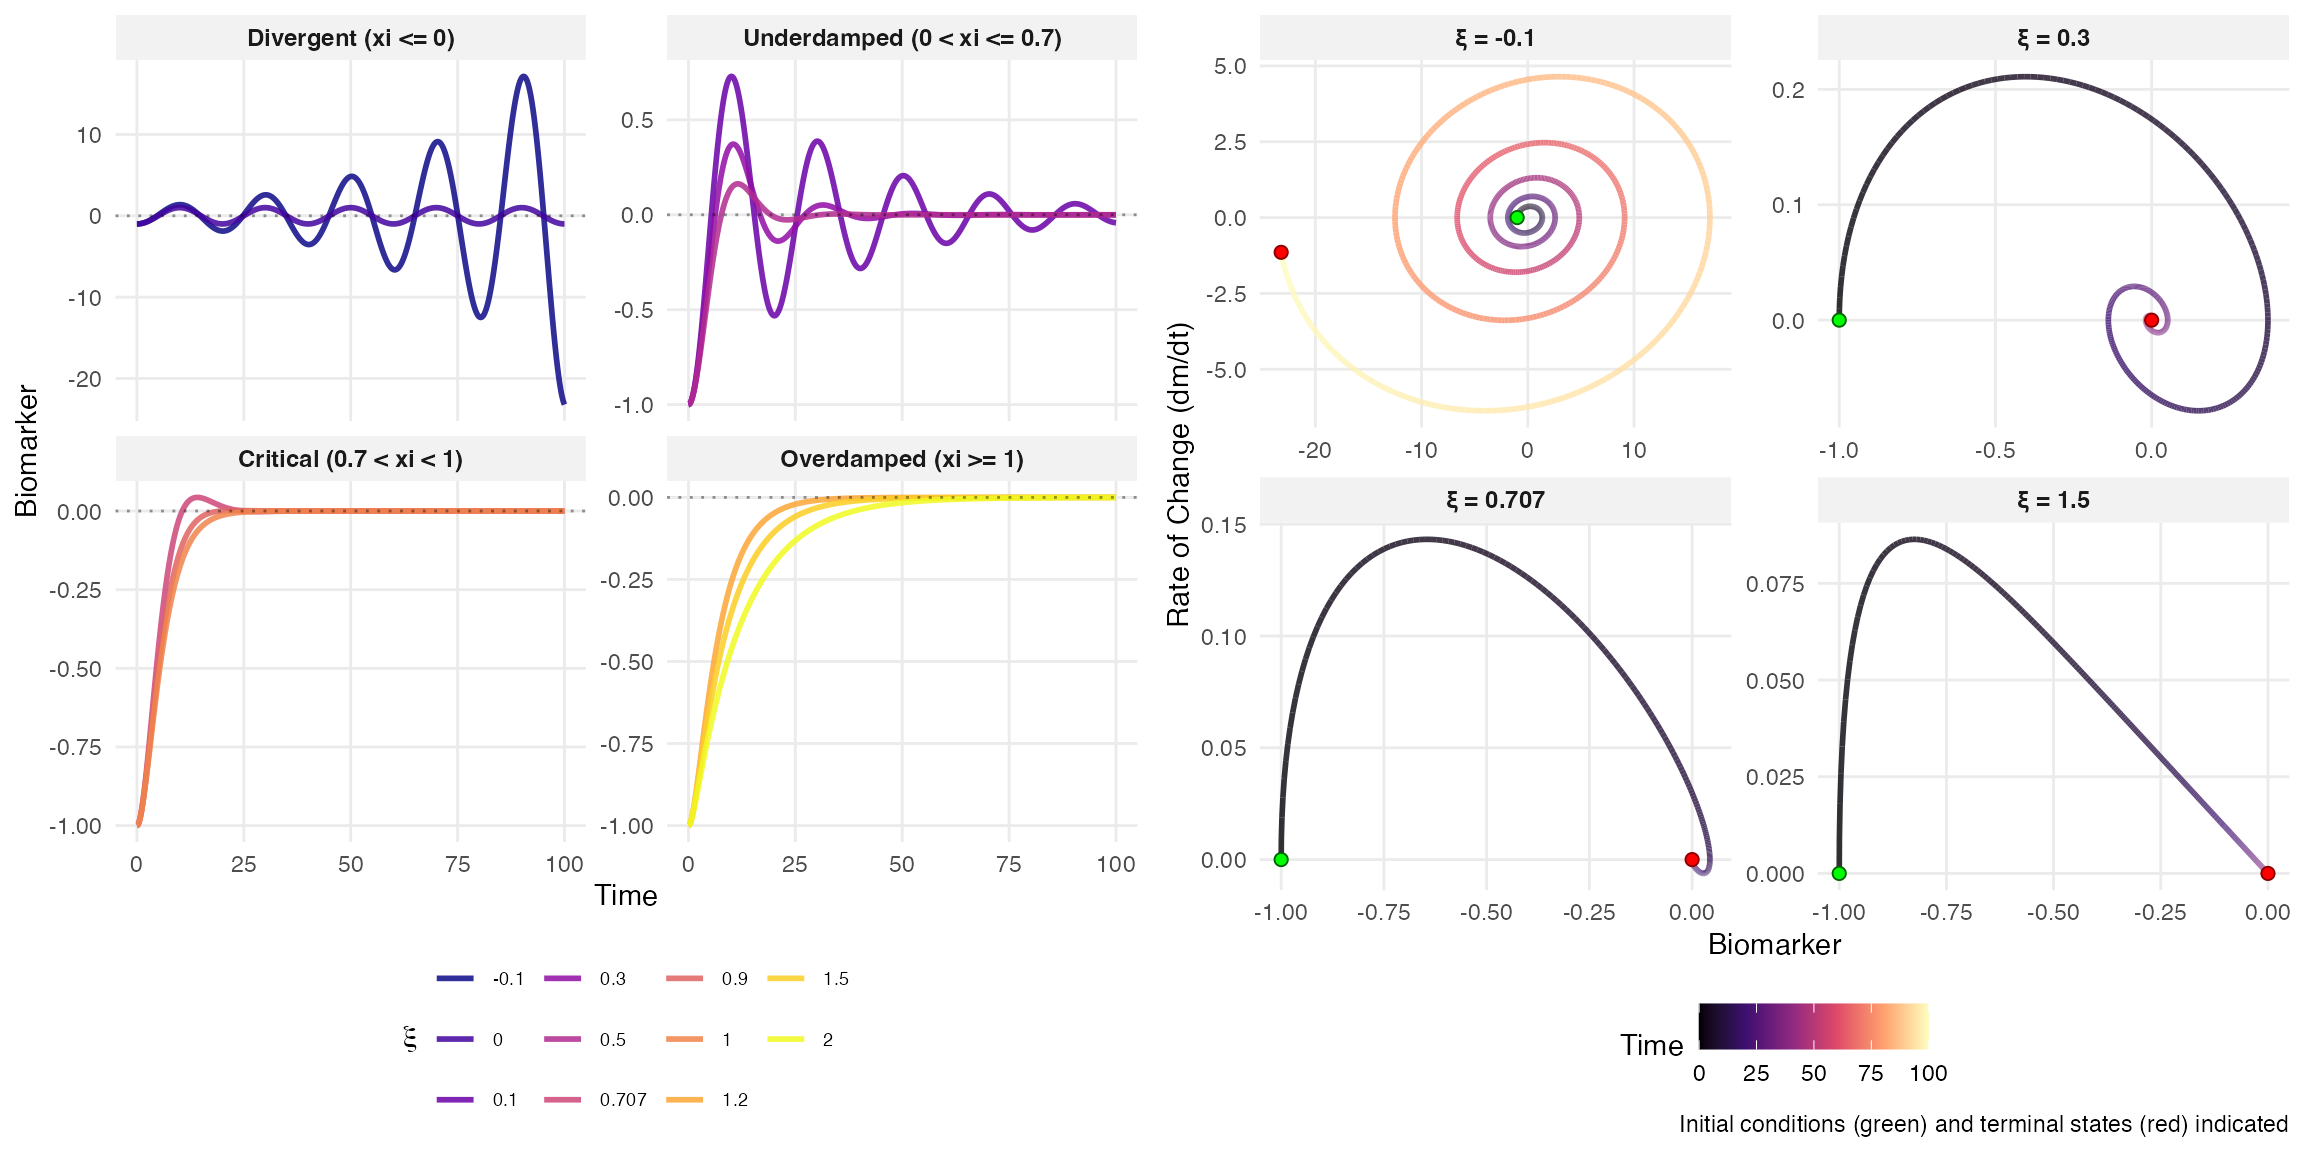
\includegraphics[width=0.85\textwidth]{../../docs/articles/illustration_files/figure-html/dynamics-plots-1.png}
    \caption{Autonomous systems with no external excitation ($u(t) = 0$)}
  \end{figure}
  \note{

    \scriptsize
    [Time: 3 min | Total: 10 min]

    Let me delve deeper into parameter interpretation. I'll focus on the stable
    case - where omega-squared is positive - as this provides the clearest
    insights.

    The figure shows the simplest scenario: an autonomous system with constant excitation u(t) equals zero.

    Starting with omega - it determines the oscillation period through the
    relationship T equals two-pi over omega. In the undamped case where xi is
    zero, you can observe complete oscillations roughly every twenty time
    units.

    Now for the damping ratio xi. The figure illustrates
    how xi values create distinct behaviors:

    When xi is negative, the system diverges exponentially with oscillations.

    For xi between zero and zero point seven, we observe decaying oscillations.

    Between zero point seven and one point zero, oscillations are minimal - just slight overshooting.

    Above one point zero, we enter the overdamped regime - monotonic convergence without any oscillation.

    The right panel is the phase plot - biomarker level versus velocity. Notice how the trajectories spiral inward for low xi, indicating oscillations, and become more direct as xi increases.
    \normalsize
  }
\end{frame}

\begin{frame}{Damping Effects (cont.)}
  \textbf{The damping ratio $\xi$ determines convergence behavior}

  \begin{table}
    \centering
    \begin{tabular}{@{}cll@{}}
      \toprule
      \textbf{Damping ($\xi$)} & \textbf{Regime} & \textbf{Behavior}                    \\
      \midrule
      $\xi \leq 0$             & Unstable        & Divergence or sustained oscillations \\
      $0 < \xi \leq 0.7$       & Underdamped     & Decaying oscillations                \\
      $0.7 < \xi < 1$          & Near-critical   & Rapid convergence, minimal overshoot \\
      $\xi \geq 1$             & Overdamped      & Slow monotonic decay                 \\
      \bottomrule
    \end{tabular}
  \end{table}

  \vspace{0.3cm}
  \textbf{Special cases:}
  \begin{itemize}
    \item $\xi = \frac{\sqrt{2}}{2} \approx 0.707$: Fastest settling time with overshoot
    \item $\xi = 1$: Critical damping, the fastest response without oscillation
  \end{itemize}
  \note{
    [Time: 2 min | Total: 12 min]

    This table summarizes the damping regimes. Each range of xi produces different dynamics.

    Two critical values deserve special attention:

    xi equals root-two over two - provides optimal settling time
    while allowing some overshoot. This is often desirable in control systems.

    xi equals one represents critical damping - the boundary between
    oscillatory and non-oscillatory behavior. It gives the fastest response
    without any oscillation.
  }
\end{frame}

\begin{frame}{External Interventions}

  \begin{figure}
    \centering
    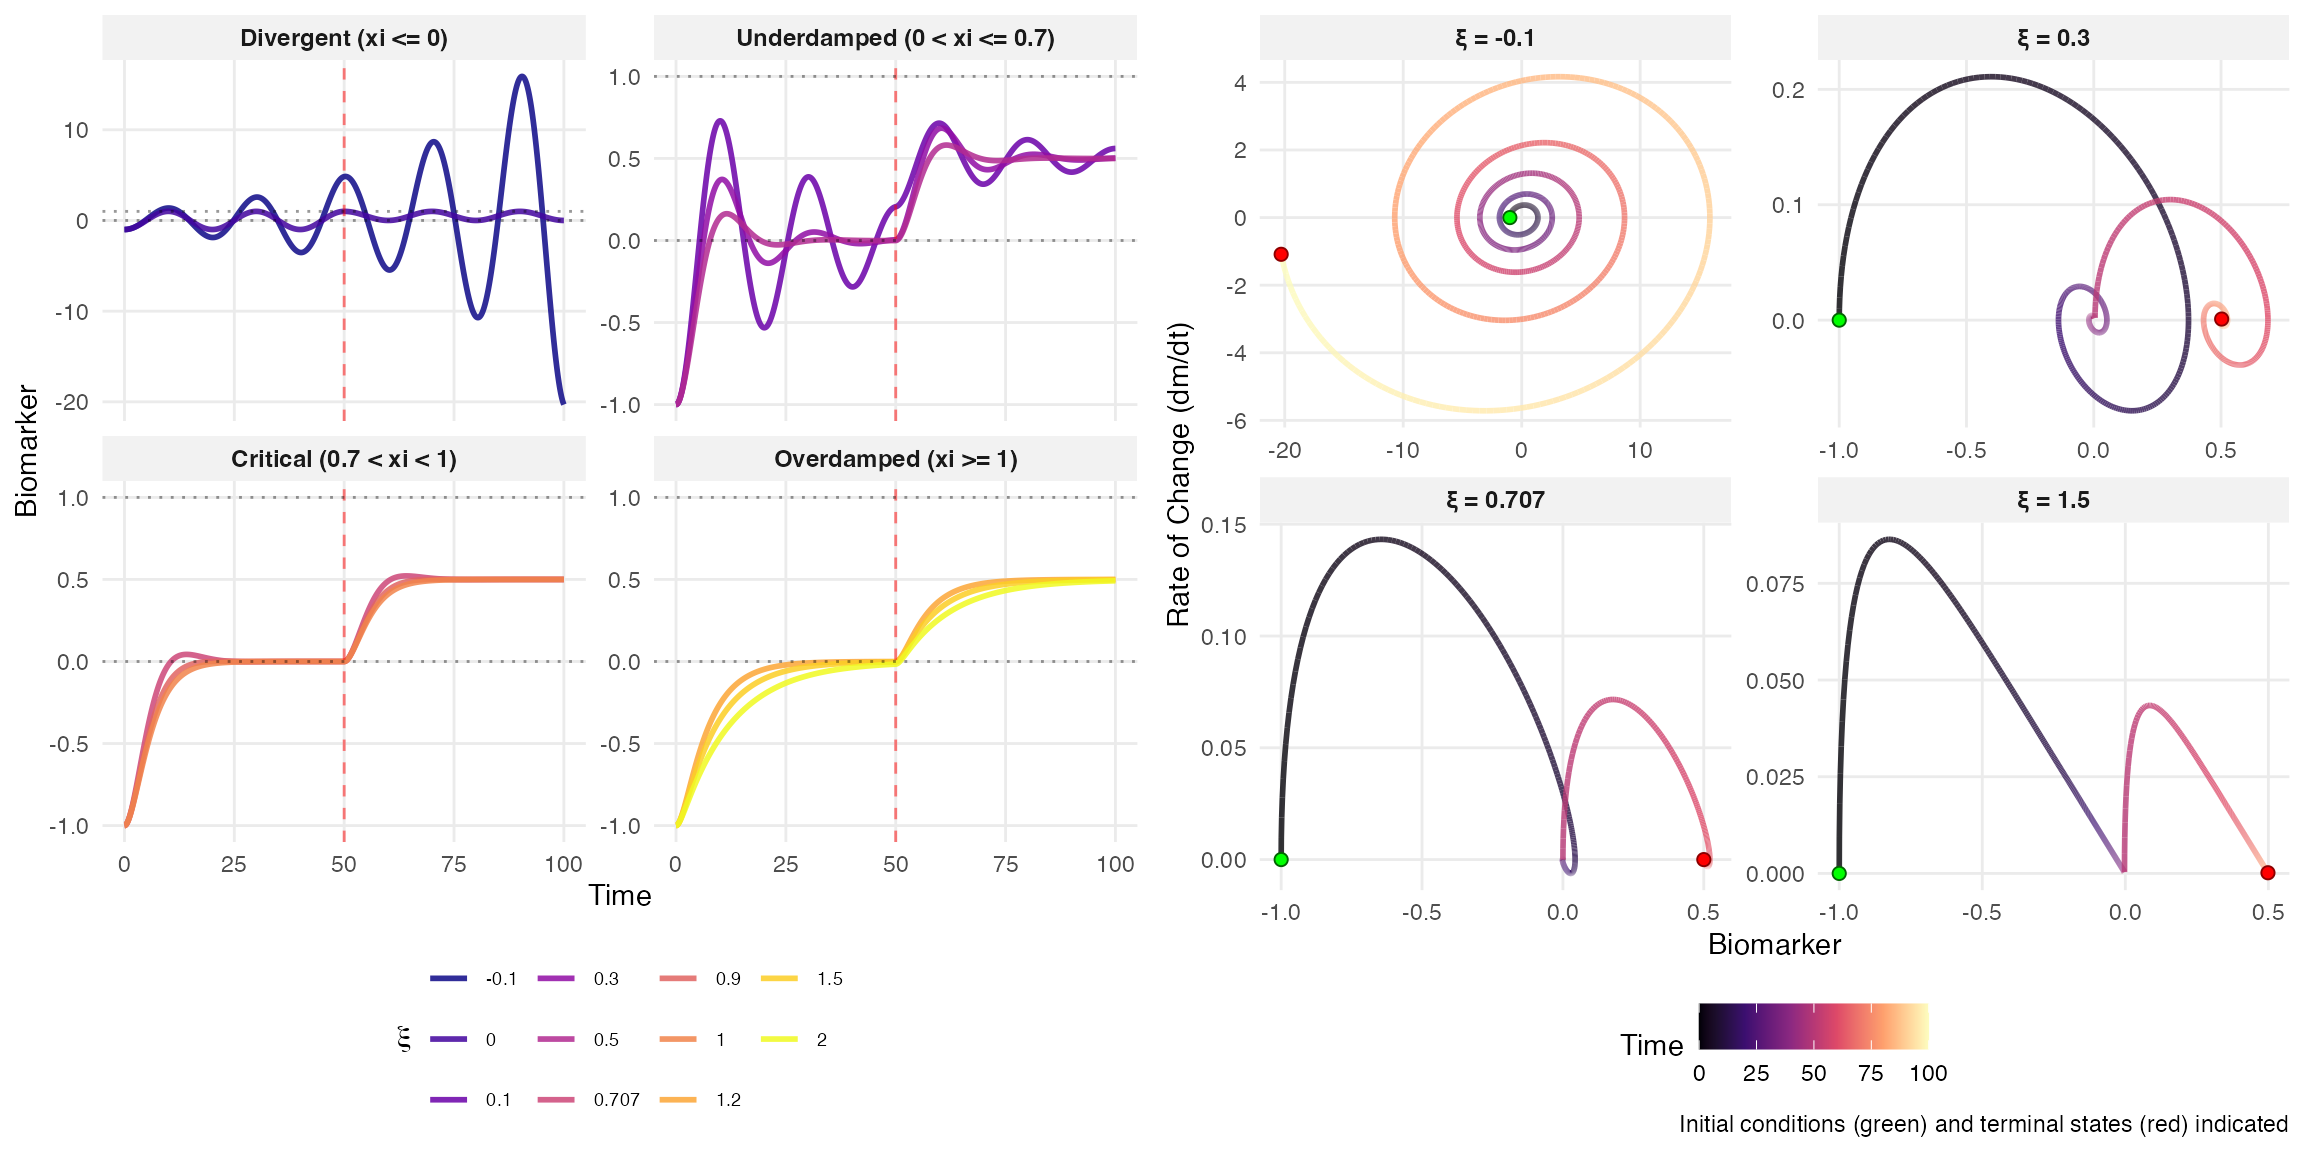
\includegraphics[width=0.75\textwidth]{../../docs/articles/illustration_files/figure-html/non-autonomous-1.png}
    \caption{Non-autonomous systems with step excitation ($u(t) = 0.5 \cdot \mathrm{I}\{t \geq 50\}$)}
  \end{figure}
  % Examples: Surgery, chemotherapy initiation, medication changes
  \note{
    [Time: 2 min | Total: 14 min]

    Now let's examine the response to external interventions - such as
    treatment change. Here, at time fifty, we introduce a step change where
    u(t) jumps from zero to zero point five.

    Notice the system's response dynamics. The new equilibrium level equals zero point five.

    Importantly, the damping ratio xi continues to govern the approach to
    equilibrium - determining whether we see oscillatory or monotonic
    convergence.

    This demonstrates how our ODE framework naturally captures real-world medical interventions - like insulin injections causing glucose levels to drop.
  }
\end{frame}

\begin{frame}{Biological Trajectories Naturally Follow ODE Dynamics}
  \begin{figure}
    \centering
    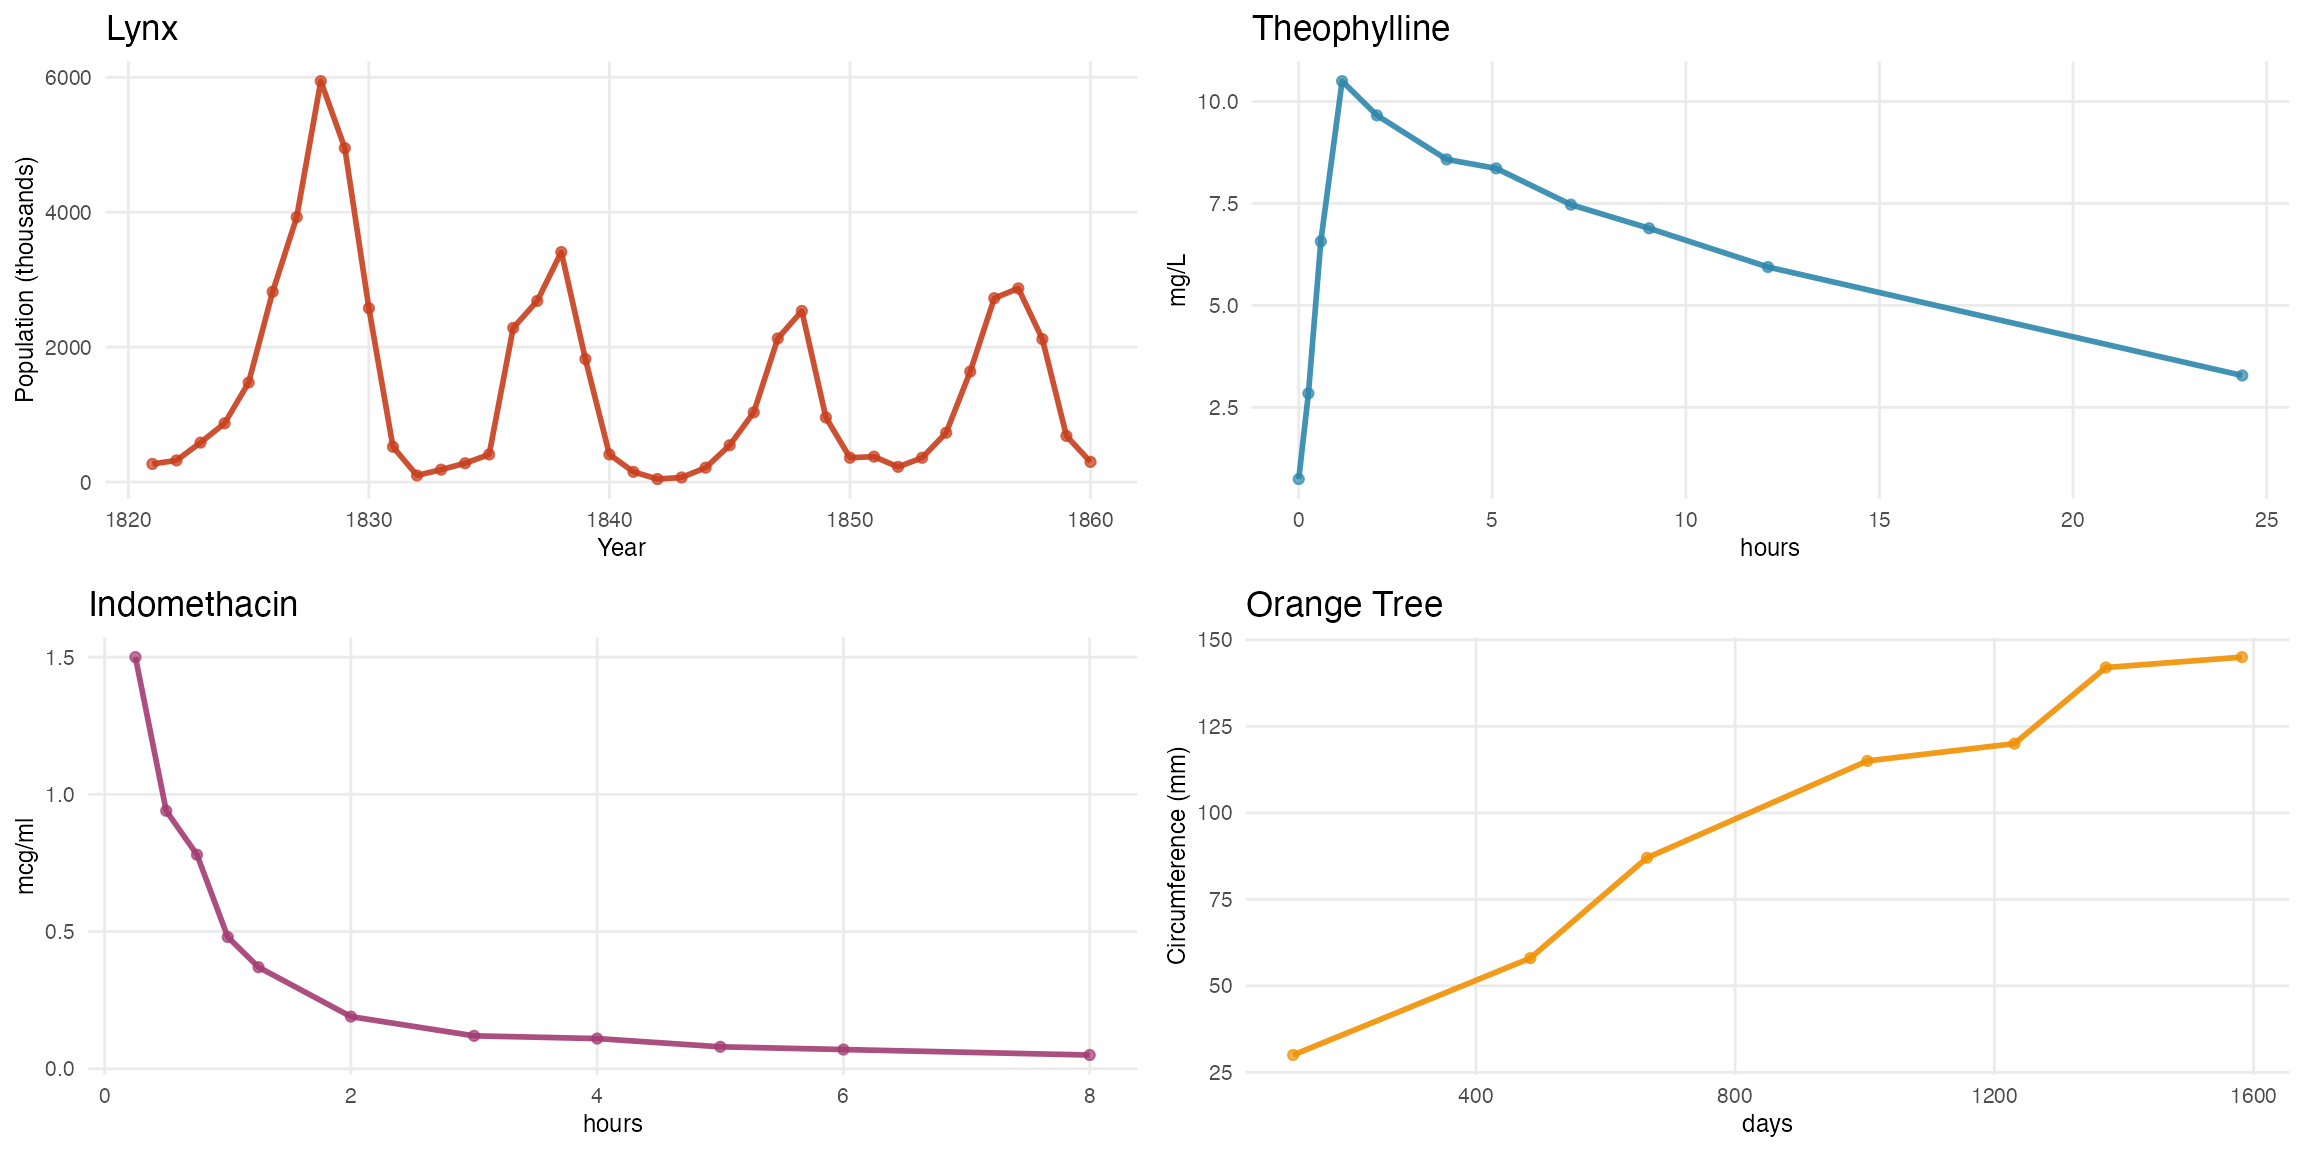
\includegraphics[width=0.7\textwidth]{../../docs/articles/illustration_files/figure-html/real-data-1.png}
    \caption{\footnotesize Diverse biological systems naturally exhibit second-order ODE dynamics. \textbf{Top-left:} Lynx population cycles. \textbf{Top-right:} Theophylline pharmacokinetics. \textbf{Bottom-left:} Indomethacin concentration. \textbf{Bottom-right:} Orange tree growth.}
  \end{figure}
  \note{
    [Time: 2 min | Total: 16 min]

    Remarkably, second-order ODE dynamics appear throughout biology and medicine.

    These examples illustrate how widespread such patterns are.
  }
\end{frame}

\section{Method}

\begin{frame}{Joint Modeling Framework}
  \structure{Longitudinal Submodel:}
  \begin{equation*}
    V_{ij} = m_i(T_{ij}) + b_i + \varepsilon_{ij}, \quad \varepsilon_{ij} \sim \mathcal{N}(0, \sigma_e^2), \quad b_i \sim \mathcal{N}(0, \sigma_b^2)
  \end{equation*}

  Biomarker dynamics governed by:
  \begin{align*}
     & \ddot{m}_i(t) + 2\xi\omega\dot{m}_i(t) + \omega^2 m_i(t) = k\omega^2 u_i(t)\Rightarrow                        \\
     & \qquad \ddot{m}_i(t) = \beta_1 m_i(t) + \beta_2 \dot{m}_i(t) + \boldsymbol{\beta}_X^{\top}\boldsymbol{X}_i(t)
  \end{align*}
  with initial conditions: $m_i(0) = m_{i0}$, $\dot{m}_i(0) = \dot{m}_{i0}$

  \vspace{0.1cm}
  \structure{Survival Submodel:}
  \begin{equation*}
    \lambda_i(t) = \lambda_0(t)\exp\Big[\underbrace{\alpha_1 m_i(t)}_{\text{level}} + \underbrace{\alpha_2\dot{m}_i^{\gamma}(t)}_{\text{volatility}} + \boldsymbol{W}_i(t)^{\top}\boldsymbol{\phi} + b_i\Big]
  \end{equation*}
  where $\gamma \in \{1, 2\}$ for linear or squared velocity effects, and $\lambda_0(t)$ is approximated by B-splines $\log(\lambda_0(t)) = \boldsymbol{\eta}^{\top}\mathbf{B}^{(\lambda)}(t)$
  \note{

    \footnotesize
    [Time: 3 min | Total: 19 min]

    With this understanding of ODE dynamics, let me outline our joint modeling framework, which consists of two
   components.

    For the longitudinal submodel, we decompose observations into the true
    trajectory plus measurement error and random effects. The trajectory evolution follows our
    second-order ODE, which we reparameterize for computational efficiency.

    The survival submodel extends traditional joint models in a key way: we
    incorporate both the biomarker level through alpha-one and its velocity
    through alpha-two. The gamma parameter allows flexibility - when gamma
    equals one, we model linear velocity effects; when gamma equals two, we
    capture volatility through squared velocity, regardless of direction, which may be more relevant in some clinical contexts, such as heart rate variability.

    We approximate the baseline hazard using B-splines to maintain flexibility.
    The entire framework is estimated via maximum likelihood, though the
    computational burden exceeds that of standard joint models.
    \normalsize
  }
\end{frame}


\begin{frame}{Unified ODE System}

  Following Tang et al. (2023)\footnotemark[3], the survival process can be naturally integrated through the relationship $\frac{d\Lambda(t)}{dt} = \lambda(t)$.

  \vspace{0.3cm}
  Define the state vector: $\boldsymbol{s}_i(t) = [\Lambda_i(t), \, m_i(t), \, \dot{m}_i(t)]^{\top}$.
  The unified system evolves as:
  \begin{equation*}
    \boxed{
      \frac{d\boldsymbol{s}_i}{dt} = \begin{pmatrix}
        \lambda_i(t|b_i) \\
        \dot{m}_i(t)     \\
        \ddot{m}_i(t)
      \end{pmatrix},\quad
      \text{with}\quad \boldsymbol{s}_i(0) = \begin{pmatrix}
        0      \\
        m_{i0} \\
        \dot{m}_{i0}
      \end{pmatrix}
    }
  \end{equation*}

  \vspace{0.3cm}
  Single ODE solver handles both longitudinal and survival processes simultaneously.

  \footnotetext[3]{\scriptsize Tang W, et al. J. Am. Stat. Assoc. 2023;118(544):2406-2421.}
  \note{
    [Time: 2.5 min | Total: 21.5 min]

    Building on Tang and colleagues' two thousand twenty-three framework, we unify both processes
    into a single ODE system.

    The crucial insight is recognizing that the cumulative hazard itself
    satisfies an ODE: d-capital-lambda/dt equals little lambda. This allows us to incorporate
    lambda as an additional state variable.

    Consequently, our state vector now comprises three components - the cumulative
    hazard, biomarker level, and biomarker velocity - all evolving
    simultaneously. A single ODE solver handles the entire system, which is
    both elegant and computationally efficient.
  }
\end{frame}

% \begin{frame}{Connection to Modern Diffusion Models\footnotemark[4]}
%   \textbf{Forward SDE:}
%   \begin{equation}
%     d\boldsymbol{x} = \underbrace{f(\boldsymbol{x}, t)}_{\text{drift}} dt + \underbrace{g(t)}_{\text{diffusion}} d\boldsymbol{w}
%   \end{equation}

%   \textbf{Reverse-time SDE:}
%   \begin{equation}
%     d\boldsymbol{x} = [\underbrace{f(\boldsymbol{x}, t)}_{\text{drift}} - \underbrace{g(t)^2 \nabla_{\boldsymbol{x}} \log p_t(\boldsymbol{x})}_{\text{score function}}] dt + g(t) d\bar{\boldsymbol{w}}
%   \end{equation}


%   This approach of modeling gradients (score function $\nabla \log p_t$ in diffusion, velocity field $\dot{m}(t)$ in our ODE) captures richer geometric and dynamic information than modeling levels directly.

%   \footnotetext[4]{\scriptsize Oko K, Akiyama S, Suzuki T. Diffusion Models are Minimax Optimal Distribution Estimators. ICML 2023.}
%   \note{
%     [Time: 2.5 min | Total: 24 min]

%     There's a fascinating connection with modern machine learning.

%     Diffusion models achieve their success by modeling gradients, specifically
%     score functions, rather than just values.

%     Our approach shares this philosophy. By explicitly modeling velocity, and we capture richer dynamic
%     information.
%   }
% \end{frame}

\begin{frame}[allowframebreaks]{Parameter Estimation: EM Algorithm}
  We employ the EM algorithm to handle the latent random effects $b_i \sim \mathcal{N}(0, \sigma_b^2)$

  \vspace{0.3cm}
  \textbf{Parameters:} $\boldsymbol{\theta} = (\omega, \xi, k, \boldsymbol{\alpha}, \boldsymbol{\beta}, \boldsymbol{\phi}, \boldsymbol{\eta}, \sigma_e^2, \sigma_b^2)$

  \textbf{Observed data:} $\mathcal{O}_i = \{(V_{ij}, T_{ij})_{j=1}^{n_i}, T_i, \delta_i\}$

  \vspace{0.3cm}
  \structure{E-step:} Given $\boldsymbol{\theta}^{(k)}$, compute posterior moments
  $$\hat{b}_i^{(k)} = E[b_i|\mathcal{O}_i; \boldsymbol{\theta}^{(k)}], \quad \hat{v}_i^{(k)} = \mathrm{Var}[b_i|\mathcal{O}_i; \boldsymbol{\theta}^{(k)}]$$

  \framebreak

  \note{
    [Time: 3 min | Total: 27 min]

    For parameter estimation, we employ the EM algorithm - the standard
    approach for joint models with latent random effects.

    In the E-step, we compute the posterior mean and variance of the random effects $b_i$ given the observed data and current parameter estimates.
  }
\end{frame}

\begin{frame}{Parameter Estimation: EM Algorithm (cont.)}
  \structure{M-step:} Maximize the expected complete-data log-likelihood
  \begin{align*}
     & Q(\boldsymbol{\theta}|\boldsymbol{\theta}^{(k)}) = E[\ell_c(\boldsymbol{\theta})|\mathcal{O}; \boldsymbol{\theta}^{(k)}] \\
     & = \sum_{i=1}^n E\Big[\log f(V_i|b_i; \boldsymbol{\theta}) + \log f(T_i, \delta_i|b_i; \boldsymbol{\theta}) + \log f(b_i; \boldsymbol{\theta})\Big|\mathcal{O}_i; \boldsymbol{\theta}^{(k)}\Big]
  \end{align*}

  Update parameters:
  $$\boldsymbol{\theta}^{(k+1)} = \arg\max_{\boldsymbol{\theta}} Q(\boldsymbol{\theta}|\boldsymbol{\theta}^{(k)})$$

  Iterate E and M steps until convergence.

  \note{
    [Time: 1 min | Total: 28 min]

    In the M-step, we maximize the expected complete-data log-likelihood
    using the posterior moments from the E-step. This yields updated parameter
    estimates.

    We iterate between E and M steps until convergence.

    The primary computational challenge lies in solving ODEs and computing
    their gradients with respect to parameters. We've developed efficient
    numerical methods to address this. For those interested in implementation
    details, I'd be happy to discuss after the presentation.
  }
  
\end{frame}

% Section 6: Results
\section{Numerical Simulations}

\begin{frame}{Simulation Design}
  \structure{Data Generation Process}
  \begin{itemize}
    \item \textbf{Sample:} $n = 100$ subjects, annual measurements per subject in $[0,10]$ years
    \item \textbf{Biomarker dynamics:} Second-order ODE with parameters
    \begin{itemize}
      \item Natural frequency: $\omega = 2\pi/5$ (period = 5 years)
      \item Damping ratio: $\xi \in \{0.7, 1.2\}$ (critical/overdamped)
    \end{itemize}
    \item \textbf{Hazard model:} $\lambda_i(t) = \lambda_0(t)\exp[\alpha_1 m_i(t) + \alpha_2 \dot{m}_i(t) + \boldsymbol{\phi}^{\top}\mathbf{W}_i + b_i]$
  \end{itemize}

  \vspace{0.3cm}
  \structure{Benchmark Comparison}
  \begin{itemize}
    \item \textbf{Proposed:} Joint ODE model estimating all parameters
    \item \textbf{Oracle:} Cox regression using true $m_i(t_j)$, $\dot{m}_i(t_j)$ at observation times
  \end{itemize}
  \note{
    [Time: 2 min | Total: 29 min]

    Let me present our simulation study, designed as a proof-of-concept for the
    proposed methodology.

    We simulated one hundred subjects over a ten-year period. As a benchmark, we compared our approach
    against an "oracle" - a Cox model with access to the true biomarker values and velocities
    at only the observation times.

    These results are preliminary. We're planning more comprehensive simulation
    studies once we better characterize real-world data patterns and identify
    relevant clinical scenarios.
  }
\end{frame}

\begin{frame}{Simulation Results (Critical Damping: $\xi = 0.7$)}
  \begin{columns}[T]
    \begin{column}{0.75\textwidth}
      \begin{table}
        \centering
        \resizebox{0.95\textwidth}{!}{%
      \begin{tabular}{ll|ccccc}
        \toprule
        \textbf{Parameter} & \textbf{Method} & \textbf{True}            & \textbf{Bias}     & \textbf{ESE}     & \textbf{ASE}     & \textbf{CP(\%)} \\
        \midrule
        \multirow{2}{*}{$\phi_1$}
                           & Oracle          & \multirow{2}{*}{$0.40$}  & $0.014$           & $0.135$          & $0.127$          & $93$            \\
                           & Proposed        &                          & $0.018$           & $0.132$          & $0.130$          & $94$            \\
        \midrule
        \multirow{2}{*}{$\phi_2$}
                           & Oracle          & \multirow{2}{*}{$-0.60$} & $-0.022$          & $0.261$          & $0.250$          & $94$            \\
                           & Proposed        &                          & $0.002$           & $0.277$          & $0.252$          & $91$            \\
        \midrule
        \multirow{2}{*}{$\alpha_1$ (level)}
                           & Oracle          & \multirow{2}{*}{$0.30$}  & $0.047$           & $0.259$          & $0.239$          & $92$            \\
                           & Proposed        &                          & $\mathbf{0.037}$  & $\mathbf{0.134}$ & $\mathbf{0.132}$ & $\mathbf{96}$   \\
        \midrule
        \multirow{2}{*}{$\alpha_2$ (velocity)}
                           & Oracle          & \multirow{2}{*}{$1.00$}  & $-0.067$          & $0.643$          & $0.585$          & $92$            \\
                           & Proposed        &                          & $\mathbf{-0.032}$ & $\mathbf{0.218}$ & $\mathbf{0.223}$ & $\mathbf{96}$   \\
        \midrule
        $T=2\pi/\omega$    & Proposed        & $5.00$                   & $0.008$           & $0.045$          & $0.039$          & $91$            \\
        $\xi$              & Proposed        & $0.70$                   & $0.000$           & $0.010$          & $0.009$          & $94$            \\
        \bottomrule
      \end{tabular}
    }
      \end{table}
    \end{column}

    \begin{column}{0.23\textwidth}
      \centering
      \footnotesize
      \textbf{Critical Damping}\\
      $\xi = 0.7$\\[0.2cm]
      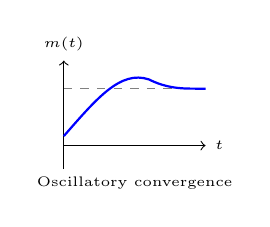
\begin{tikzpicture}[scale=0.6]
        \draw[->] (0,0) -- (3,0) node[right] {\tiny $t$};
        \draw[->] (0,-0.5) -- (0,1.8) node[above] {\tiny $m(t)$};
        \draw[dashed,gray] (0,1.2) -- (3,1.2);
        \draw[thick,blue] (0,0.2) .. controls (0.7,1.0) and (1.2,1.6) .. (1.8,1.4) .. controls (2.3,1.15) and (2.7,1.22) .. (3,1.2);
        \node at (1.5,-0.8) {\tiny Oscillatory convergence};
      \end{tikzpicture}
    \end{column}
  \end{columns}

  \vspace{0.1cm}
  \footnotesize
  \textbf{Note:} ESE: empirical SE; ASE: asymptotic SE; CP: coverage probability.
  \note{

    \small
    [Time: 3 min | Total: 32 min]

    We first examine the critical damping scenario with xi equals zero point seven. The true biomarker trajectory converges fast to equilibrium with some overshoot.

    The results reveal an interesting pattern. For covariates phi-one
    and phi-two, our method performs comparably to the oracle - as expected,
    since these don't involve the ODE structure.
    But examine the biomarker effects. Our standard errors are
    smaller than the oracle's. For the level effect alpha-one: zero point one three four versus
    zero point two five nine. For the velocity effect alpha-two: zero point two one eight versus zero point six four three.

    What drives this efficiency gain? The oracle only observes discrete
    snapshots at observation times. In contrast, our ODE framework models the
    entire continuous trajectory, effectively interpolating between
    observations.
    \normalsize
  }
\end{frame}

\begin{frame}{Simulation Results (Overdamped: $\xi = 1.2$)}
  \begin{columns}[T]
    \begin{column}{0.75\textwidth}
      \begin{table}
        \centering
        \resizebox{0.95\textwidth}{!}{%
      \begin{tabular}{ll|ccccc}
        \toprule
        \textbf{Parameter} & \textbf{Method} & \textbf{True}            & \textbf{Bias}     & \textbf{ESE}     & \textbf{ASE}     & \textbf{CP(\%)} \\
        \midrule
        \multirow{2}{*}{$\phi_1$}
                           & Oracle          & \multirow{2}{*}{$0.40$}  & $0.011$           & $0.136$          & $0.131$          & $93$            \\
                           & Proposed        &                          & $0.015$           & $0.136$          & $0.134$          & $94$            \\
        \midrule
        \multirow{2}{*}{$\phi_2$}
                           & Oracle          & \multirow{2}{*}{$-0.60$} & $-0.033$          & $0.276$          & $0.258$          & $92$            \\
                           & Proposed        &                          & $-0.023$          & $0.280$          & $0.260$          & $92$            \\
        \midrule
        \multirow{2}{*}{$\alpha_1$ (level)}
                           & Oracle          & \multirow{2}{*}{$0.30$}  & $0.040$           & $0.258$          & $0.238$          & $92$            \\
                           & Proposed        &                          & $\mathbf{0.042}$  & $\mathbf{0.159}$ & $\mathbf{0.151}$ & $\mathbf{94}$   \\
        \midrule
        \multirow{2}{*}{$\alpha_2$ (velocity)}
                           & Oracle          & \multirow{2}{*}{$1.00$}  & $-0.105$          & $1.070$          & $0.943$          & $90$            \\
                           & Proposed        &                          & $\mathbf{-0.138}$ & $\mathbf{0.449}$ & $\mathbf{0.412}$ & $\mathbf{94}$   \\
        \midrule
        $T=2\pi/\omega$    & Proposed        & $5.00$                   & $0.015$           & $0.086$          & $0.083$          & $92$            \\
        $\xi$              & Proposed        & $1.20$                   & $-0.003$          & $0.026$          & $0.027$          & $94$            \\
        \bottomrule
      \end{tabular}
    }
      \end{table}
    \end{column}

    \begin{column}{0.23\textwidth}
      \centering
      \footnotesize
      \textbf{Overdamped}\\
      $\xi = 1.2$\\[0.2cm]
      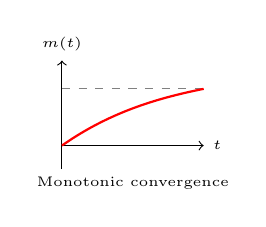
\begin{tikzpicture}[scale=0.6]
        \draw[->] (0,0) -- (3,0) node[right] {\tiny $t$};
        \draw[->] (0,-0.5) -- (0,1.8) node[above] {\tiny $m(t)$};
        \draw[dashed,gray] (0,1.2) -- (3,1.2);
        \draw[thick,red] (0,0) .. controls (1,0.7) and (2,1.0) .. (3,1.2);
        \node at (1.5,-0.8) {\tiny Monotonic convergence};
      \end{tikzpicture}
    \end{column}
  \end{columns}

  \vspace{0.1cm}
  \footnotesize
  \textbf{Note:} ESE: empirical SE; ASE: asymptotic SE; CP: coverage probability.
  \note{
    [Time: 2 min | Total: 34 min]

    Here are the results for the overdamped settings, where xi equals one point two. The biomarker
    converges slowly and monotonically to equilibrium.

    The overdamped scenario exhibits similar efficiency gains for biomarker effects.

    However, note that velocity estimation becomes more challenging - the
    standard errors for alpha-two are larger than in the critical damping case.
    This is intuitive: slowly evolving systems provide less information about
    rates of change.
  }
\end{frame}

\begin{frame}{Extrapolation Capability of Proposed Method}
  \begin{figure}
    \centering
    
\includegraphics[width=0.9\textwidth]{man/figures/README-visualization-1.png}
  \end{figure}
  \begin{center}
    The ODE-based approach enables principled extrapolation beyond observed time window
  \end{center}
  \note{
    [Time: 2 min | Total: 36 min]

    A notable advantage of the ODE framework is its natural extrapolation
    capability. Since we model the mechanistic dynamics, we can predict biomarker
    levels and velocities even beyond the observed time window.

    This figure demonstrates individual trajectory predictions from our model.
    Observe how the framework provides extrapolation beyond the observation window.
  }
\end{frame}


% Section 5: Conclusions
\section{Conclusions}

\begin{frame}{Summary}
  \structure{Methodological Innovation:}
  \begin{enumerate}
    \item Mechanistic modeling of biomarker trajectories via second-order ODEs
    \item Natural incorporation of velocity
  \end{enumerate}

  \vspace{0.5cm}
  \structure{Future Directions:}
  \begin{itemize}
    \item \textbf{Heterogeneous dynamics:} Allow patient-specific $\omega$ and $\xi$ parameters to capture population heterogeneity
    \item \textbf{Variable selection:} Develop methods for selecting informative biomarkers when multiple candidates are available
    \item \textbf{Biomarker interactions:} Model cross-talk and feedback loops between multiple biomarkers via coupled ODEs
  \end{itemize}
  \note{
    [Time: 2.5 min | Total: 38.5 min]

    Let me summarize our current work and future directions.

    We've developed a mechanistic joint modeling framework using second-order
    ODEs that offers several advantages:
    - natural incorporation of biomarker velocity
    - interpretable parameters with physical meaning

    Our future research will focus on three areas: allowing patient-specific
    dynamic parameters, extending to multiple correlated biomarkers, and
    identifying specific clinical contexts where velocity information provides
    the greatest predictive value.
  }
\end{frame}

\begin{frame}{Computational Challenges}
  \structure{Individual ODE Solutions}
  \begin{itemize}
    \item Each patient requires solving their own ODE system
    \item Computational cost scales linearly with sample size: $\mathcal{O}(n)$
  \end{itemize}

  \vspace{0.5cm}
  \structure{Gradient Computation via Augmented ODEs}
  \begin{itemize}
    \item Computing $\nabla_{\boldsymbol{\theta}} \mathcal{L}$ requires solving an augmented system:
          \begin{equation*}
            \frac{d}{dt}\begin{pmatrix} \boldsymbol{s}(t) \\ \frac{\partial \boldsymbol{s}}{\partial \boldsymbol{\theta}} \end{pmatrix} = \begin{pmatrix} f(\boldsymbol{s}, \boldsymbol{\theta}, t) \\ \frac{\partial f}{\partial \boldsymbol{s}} \frac{\partial \boldsymbol{s}}{\partial \boldsymbol{\theta}} + \frac{\partial f}{\partial \boldsymbol{\theta}} \end{pmatrix}
          \end{equation*}
    \item Dimension grows from $d$ to $d(1 + p)$ where $p$ = number of parameters
    \item Significant memory and computation overhead
  \end{itemize}
  \note{

    \footnotesize
    [Time: 2.5 min | Total: 41 min]

    I should address the computational challenges inherent in this approach.

    First, scalability: each patient requires solving their own ODE system,
    leading to O(N) computational complexity. For large cohort studies, this
    can become prohibitive.

    Second, gradient computation: to optimize the likelihood, we must compute
    nabla (pronounced "NAB-lah") theta L, which requires solving augmented ODE
    systems that track both states and their parameter sensitivities.

    This augmentation increases the system dimension from D to D times (one plus
    P), where P is the number of parameters. For complex models, this creates
    substantial computational overhead.

    We're actively investigating several solutions: parallelization across
    patients, adaptive ODE solvers that adjust precision dynamically, and
    automatic differentiation frameworks that may provide more efficient
    gradient computation.
    \normalsize
  }
\end{frame}

\begin{frame}{Thank You}
  \begin{center}
    \Huge Questions \& Discussion
  \end{center}

  \vspace{0.8cm}

  \begin{center}
    \normalsize
    \textbf{Resources:}\\[0.3cm]
    \url{github.com/ziyangg98/JointODE}\\[0.2cm]
  \end{center}

  \vspace{0.8cm}

  \begin{center}
    \large \textit{Thank you for your attention and feedback}
  \end{center}
  \note{

    \footnotesize
    [Time: 2 min | Total: 43 min + Q&A]

    Thank you for your attention.

    Our code is publicly available on GitHub at GitHub dot com slash ziyangg ninety-eight slash joint ODE.
    We're currently preparing a manuscript with full technical details.

    I welcome any questions about the methodology, computational aspects, or
    potential applications to your own research problems.

    [Be prepared for questions on:
    - How to initialize the EM algorithm
    - Handling missing data patterns
    - Extension to multiple biomarkers
    - Computational efficiency strategies
    - Software implementation details
    - Performance versus standard joint models]
    \normalsize
  }
\end{frame}

% Appendix
\appendix

\begin{frame}{Appendix: ODE Solution Forms and Damping Behaviors}
  \begin{table}
    \centering
    \resizebox{0.95\textwidth}{!}{%
    \begin{tabular}{@{}llll@{}}
      \toprule
      \textbf{Damping} & \textbf{Condition} & \textbf{Solution Form} & \textbf{Behavior} \\
      \midrule
      Underdamped & $0 < \xi < 1$ & $e^{-\xi\omega t}[A\cos(\omega_d t) + B\sin(\omega_d t)]$ & Decaying oscillations \\
      Critical & $\xi = 1$ & $(A + Bt)e^{-\omega t}$ & Fastest decay \\
      Overdamped & $\xi > 1$ & $Ae^{\lambda_1 t} + Be^{\lambda_2 t}$ & Slow decay \\
      Undamped & $\xi = 0$ & $A\cos(\omega t) + B\sin(\omega t)$ & Sustained oscillations \\
      Unstable & $\omega^2 < 0$ or $\omega\xi < 0$ & Exponential growth & System diverges \\
      \bottomrule
    \end{tabular}
    }
  \end{table}

  \vspace{0.3cm}
  \begin{itemize}
    \item $\omega_d = \omega\sqrt{1 - \xi^2}$: damped natural frequency
    \item $\lambda_{1,2} = -\xi\omega \pm \omega\sqrt{\xi^2 - 1}$: overdamped eigenvalues
    \item $A, B$: constants determined by initial conditions $m_0, \dot{m}_0$
  \end{itemize}
  \note{

    \footnotesize
    [Time: 2 min if asked]

    [If asked about mathematical details]

    This table shows the analytical solution forms for different damping regimes.

    For underdamped systems where xi is between zero and one, we get e to the
    negative xi-omega-t [read: e to the negative xi omega t] times oscillating
    terms with cosine and sine of omega-d-t [read: omega d t].

    Critical damping at xi equals one gives the fastest decay without oscillation.

    Overdamped systems have two real eigenvalues lambda-one and lambda-two
    [read: lambda one and lambda two].

    The damped natural frequency omega-d equals omega times square root of one
    minus xi-squared [read: omega d equals omega times square root of one minus
    xi squared].
    \normalsize
  }
\end{frame}

\begin{frame}{Appendix: Model Reparameterization}

  We reparameterize the ODE for easier estimation:

  $$\ddot{m}(t) + 2\xi\omega\dot{m}(t) + \omega^2 m(t) = k\omega^2 u(t)$$

  $$\Downarrow \text{ Reparameterization}$$

  $$\ddot{m}(t) = \beta_1 m(t) + \beta_2 \dot{m}(t) + \boldsymbol{\beta}_X^{\top}\mathbf{X}(t)$$

  \vspace{0.4cm}
  \textbf{Parameter Recovery:}
  \begin{center}
    \begin{tabular}{lcl}
      $\omega$ & $=$ & $\sqrt{-\beta_1}$                                                                                                       \\
      $\xi$    & $=$ & $-\beta_2/(2\sqrt{-\beta_1})$                                                                                           \\
      SE       & via & Delta method: $\nabla g(\boldsymbol{\beta})^{\top} \mathrm{Var}(\hat{\boldsymbol{\beta}}) \nabla g(\boldsymbol{\beta})$
    \end{tabular}
  \end{center}
  \note{

    \footnotesize
    [Time: 2 min if asked]

    [If asked about parameter estimation details]

    We reparameterize the ODE for easier estimation. The original form has
    products like two-xi-omega [read: two xi omega] which are hard to optimize.

    After reparameterization, beta-one equals negative omega-squared [read:
    beta one equals negative omega squared], and beta-two equals negative two-
    xi-omega [read: beta two equals negative two xi omega].

    To recover the original parameters: omega equals square root of negative
    beta-one [read: omega equals square root of negative beta one], and xi
    equals negative beta-two over two times square root of negative beta-one
    [read: xi equals negative beta two over two times square root of negative
    beta one].

    Standard errors are computed via the delta method using the gradient of the
    transformation.
    \normalsize
  }
\end{frame}

\begin{frame}{Appendix: EM Algorithm}
  \begin{enumerate}
    \item \textbf{Initialization:} Set $\boldsymbol{\theta}^{(0)}$, $k \leftarrow 0$

          \vspace{0.2cm}
    \item \textbf{Main Loop:}
          \begin{itemize}
            \item[2a.] \textit{ODE phase:} For each patient $i$
                  \begin{itemize}
                    \item Solve augmented ODE system $\rightarrow$ $(m_i, \frac{\partial m_i}{\partial \boldsymbol{\theta}})$
                    \item Compute hazard components
                  \end{itemize}
            \item[2b.] \textit{Posterior phase:} Compute $\hat{b}_i$, $E[e^{b_i}]$
            \item[2c.] \textit{Gradient phase:} Evaluate $\nabla_{\boldsymbol{\theta}} Q$
            \item[2d.] \textit{Update:} $\boldsymbol{\theta}^{(k+1)} \leftarrow$ L-BFGS-B step
          \end{itemize}

          \vspace{0.2cm}
    \item \textbf{Convergence:} $\|\nabla Q\| < 10^{-4}$ or $|\Delta Q| < 10^{-6}$
  \end{enumerate}
  \note{

    \footnotesize
    [Time: 2-3 min if asked]

    [If asked about algorithm details]

    Here's our EM algorithm structure.

    We initialize parameters theta-zero [read: theta naught] using method of
    moments or simple mixed models.

    In each iteration:
    First, the ODE phase solves the augmented system for each patient to get
    trajectories (tra-JECK-tor-eez) and sensitivities.
    Second, the posterior phase computes b-hat-i [read: b hat sub i] and the
    expectation of e to the b-i [read: e to the b sub i].
    Third, we evaluate gradients of the Q function.
    Fourth, we update using L-BFGS-B, a limited-memory quasi-Newton method.

    We converge when the gradient norm is less than ten to the minus four
    [read: ten to the minus four] or the change in Q is less than ten to the
    minus six [read: ten to the minus six].
    \normalsize
  }
\end{frame}

\begin{frame}{Appendix: Posterior Computation}
  \structure{Key Insight - Factorization:}
  $$\lambda_i(t|b_i) = e^{b_i} \lambda_i(t|0), \quad \Lambda_i(t|b_i) = e^{b_i} \Lambda_i(t|0)$$

  \vspace{0.3cm}
  \structure{Computational Strategy:}
  \begin{enumerate}
    \item Solve ODE once with $b_i = 0$ to get $\Lambda_i(t|0)$
    \item Find posterior mode by maximizing:
          $$\ell_i(b) = b\left[\frac{S_i}{\sigma_e^2} + \delta_i\right] - \frac{b^2}{2}\left[\frac{n_i}{\sigma_e^2} + \frac{1}{\sigma_b^2}\right] - e^b\Lambda_i(T_i|0)$$
          where $S_i = \sum_j(V_{ij} - m_i(T_{ij}))$
    \item Compute moments via Gauss-Hermite quadrature
  \end{enumerate}
  \note{

    \small
    [Time: 2 min if asked]

    [If asked about computational efficiency]

    The key insight is factorization - the hazard with random effect b-i equals
    e to the b-i [read: e to the b sub i] times the hazard at b-i equals zero.

    This allows us to:
    First, solve the ODE once with b-i equals zero.
    Second, find the posterior mode by maximizing this log-posterior, where s-i
    [read: S sub i] is the sum of residuals.
    Third, compute moments using Gauss-Hermite quadrature around the mode.

    This factorization dramatically reduces computation - we don't need to re-
    solve ODEs for different b-i values.
    \normalsize
  }
\end{frame}

\begin{frame}{Appendix: Gradient-Based Optimization}
  \structure{Objective:} Maximize $Q(\boldsymbol{\theta})$ where $\boldsymbol{\theta} = (\boldsymbol{\eta}, \boldsymbol{\phi}, \boldsymbol{\alpha}, \boldsymbol{\beta}, \sigma_e^2, \sigma_b^2)$

  \vspace{0.3cm}
  \structure{Gradient Decomposition:}
  $$\nabla_{\boldsymbol{\theta}} Q = \underbrace{\sum_{i,j} \frac{r_{ij}}{\sigma_e^2} \frac{\partial m_i(T_{ij})}{\partial \boldsymbol{\theta}}}_{\text{Longitudinal component}} + \underbrace{\sum_i \left[\delta_i \frac{\partial \log\lambda_i}{\partial \boldsymbol{\theta}} - E[e^{b_i}] \frac{\partial \Lambda_i}{\partial \boldsymbol{\theta}}\right]}_{\text{Survival component}}$$
  where $r_{ij} = V_{ij} - m_i(T_{ij}) - \hat{b}_i$ is the residual

  \vspace{0.3cm}
  \begin{center}
    No analytical form $\rightarrow$ numerical computation required
  \end{center}
  \note{

    \small
    [Time: 2 min if asked]

    [If asked about optimization details]

    The gradient of Q decomposes into two parts.

    The longitudinal component involves residuals r-i-j [read: r sub i j]
    weighted by one over sigma-e-squared, times the trajectory sensitivities.

    The survival component has the event indicator delta-i times the log-hazard
    gradient, minus the expected cumulative hazard gradient.

    Since we don't have analytical forms for the ODE solutions, all gradients
    must be computed numerically by solving the augmented ODE system.
    \normalsize
  }
\end{frame}

\begin{frame}{Appendix: Gradient-Based Computation cont.}
  \structure{Strategy:} Solve state and sensitivities Simultaneously
  \vspace{0.3cm}

  Denote $\mathbf{Z}_i(t) = [m_i(t), \dot{m}_i(t), \mathbf{X}_i(t)^{\top}]^{\top}$, then the augmented system is:
  $$\frac{d}{dt}\begin{pmatrix}
      \Lambda_i(t)                                            \\
      m_i(t)                                                  \\
      \dot{m}_i(t)                                            \\
      \frac{\partial \Lambda_i}{\partial \boldsymbol{\beta}} \\
      \frac{\partial m_i}{\partial \boldsymbol{\beta}}       \\
      \frac{\partial \dot{m}_i}{\partial \boldsymbol{\beta}}
    \end{pmatrix} = \begin{pmatrix}
      \lambda_i(t|0)                                                                                                                                            \\
      \dot{m}_i(t)                                                                                                                                              \\
      \boldsymbol{\beta}^{\top}\mathbf{Z}_i(t)                                                                                                                  \\
      \frac{\partial \lambda_i}{\partial \boldsymbol{\beta}} + \lambda_i \boldsymbol{\alpha}^{\top} \frac{\partial \mathbf{m}_i}{\partial \boldsymbol{\beta}} \\
      \frac{\partial \dot{m}_i}{\partial \boldsymbol{\beta}}                                                                                                   \\
      \mathbf{Z}_i(t) + \boldsymbol{\beta}^{\top}\frac{\partial \mathbf{Z}_i(t)}{\partial \boldsymbol{\beta}}
    \end{pmatrix}$$

  Initial State $(0, m_{i0}, \dot{m}_{i0})$, Sensitivities all zero
  \note{

    \footnotesize
    [Time: 2-3 min if asked]

    [If asked about implementation details]

    We solve states and sensitivities simultaneously in one augmented ODE system.

    The state vector z-i [read: Z sub i] contains the biomarker level,
    velocity, and covariates.

    The augmented system has the original three states plus their sensitivities
    with respect to all parameters.

    The initial state starts at zero for cumulative hazard, m-i-zero and m-dot-
    i-zero [read: m sub i naught and m dot sub i naught] for the biomarker.

    All sensitivities start at zero since initial conditions don't depend on
    parameters.

    This approach is more efficient than finite differences and provides exact
    gradients up to ODE solver tolerance.
    \normalsize
  }
\end{frame}

\end{document}